\documentclass[11pt,professionalfonts,hyperref={pdftex,pdfpagemode=none,pdfstartview=FitH}]{beamer}
%\usepackage{times}
%\usefonttheme{serif}
%\usepackage{helvet}
%\usepackage{amsmath,amssymb}
\usepackage{graphicx,multirow}
%\usepackage[scriptsize]{subfigure}
\usepackage{subcaption}
%\usepackage{media9}
\usepackage{movie15}
\usepackage{hyperref}


%\usepackage{warmread}
%\usepackage[all,import]{xy}

%\renewcommand\mathfamilydefault{\rmdefault}

\newcommand{\norm}[1]{\ensuremath{\left\| #1 \right\|}}
\newcommand{\bracket}[1]{\ensuremath{\left[ #1 \right]}}
\newcommand{\braces}[1]{\ensuremath{\left\{ #1 \right\}}}
\newcommand{\parenth}[1]{\ensuremath{\left( #1 \right)}}
\newcommand{\pair}[1]{\ensuremath{\langle #1 \rangle}}
\newcommand{\met}[1]{\ensuremath{\langle\langle #1 \rangle\rangle}}
\newcommand{\refeqn}[1]{(\ref{eqn:#1})}
\newcommand{\reffig}[1]{Fig. \ref{fig:#1}}
\newcommand{\tr}[1]{\mathrm{tr}\ensuremath{\negthickspace\bracket{#1}}}
\newcommand{\trs}[1]{\mathrm{tr}\ensuremath{[#1]}}
\newcommand{\deriv}[2]{\ensuremath{\frac{\partial #1}{\partial #2}}}
\newcommand{\SO}{\ensuremath{\mathsf{SO(3)}}}
\newcommand{\T}{\ensuremath{\mathsf{T}}}
\renewcommand{\L}{\ensuremath{\mathsf{L}}}
\newcommand{\so}{\ensuremath{\mathfrak{so}(3)}}
\newcommand{\SE}{\ensuremath{\mathsf{SE(3)}}}
\newcommand{\se}{\ensuremath{\mathfrak{se}(3)}}
\renewcommand{\Re}{\ensuremath{\mathbb{R}}}
\newcommand{\aSE}[2]{\ensuremath{\begin{bmatrix}#1&#2\\0&1\end{bmatrix}}}
\newcommand{\ase}[2]{\ensuremath{\begin{bmatrix}#1&#2\\0&0\end{bmatrix}}}
\newcommand{\D}{\ensuremath{\mathbf{D}}}
\newcommand{\Sph}{\ensuremath{\mathsf{S}}}
\renewcommand{\S}{\Sph}
\newcommand{\J}{\ensuremath{\mathbf{J}}}
\newcommand{\Ad}{\ensuremath{\mathrm{Ad}}}
\newcommand{\intp}{\ensuremath{\mathbf{i}}}
\newcommand{\extd}{\ensuremath{\mathbf{d}}}
\newcommand{\hor}{\ensuremath{\mathrm{hor}}}
\newcommand{\ver}{\ensuremath{\mathrm{ver}}}
\newcommand{\dyn}{\ensuremath{\mathrm{dyn}}}
\newcommand{\geo}{\ensuremath{\mathrm{geo}}}
\newcommand{\Q}{\ensuremath{\mathsf{Q}}}
\newcommand{\G}{\ensuremath{\mathsf{G}}}
\newcommand{\g}{\ensuremath{\mathfrak{g}}}
\newcommand{\Hess}{\ensuremath{\mathrm{Hess}}}
\newcommand{\refprop}[1]{Proposition \ref{prop:#1}}
\newcommand{\argmin}{\operatornamewithlimits{argmin}}
\newcommand{\argmax}{\operatornamewithlimits{argmax}}

\definecolor{mygray}{gray}{0.9}

\mode<presentation> {
  \usetheme{Warsaw}
  \usefonttheme{serif}
  \setbeamercovered{transparent}
}

\newcommand{\mypaper}{}

\setbeamertemplate{footline}%{split theme}
{%
  \leavevmode%
  \hbox{\begin{beamercolorbox}[wd=.85\paperwidth,ht=2.5ex,dp=1.125ex,leftskip=.3cm,rightskip=.3cm plus1fill]{author in head/foot}%
    \usebeamerfont{author in head/foot}\insertshorttitle
  \end{beamercolorbox}%
  \begin{beamercolorbox}[wd=.15\paperwidth,ht=2.5ex,dp=1.125ex,leftskip=.3cm,rightskip=.3cm]{title in head/foot}
    \usebeamerfont{title in head/foot}\mypaper\hfill \insertframenumber/\inserttotalframenumber
%    \usebeamerfont{title in head/foot}\hfill \insertframenumber/\inserttotalframenumber
  \end{beamercolorbox}}%
  \vskip0pt%
} \setbeamercolor{box}{fg=black,bg=yellow}

\title[Autonomous Quadrotor 3D Mapping and Exploration Using Exact Occupancy Probabilities]{\large Autonomous Quadrotor 3D Mapping and Exploration Using Exact Occupancy Probabilities}

\author{\vspace*{-0.3cm}}

\institute{\footnotesize
{\normalsize Evan Kaufman, Kuya Takami,\\Zhuming Ai, and Taeyoung Lee}\vspace*{0.2cm}\\
  Mechanical and Aerospace Engineering\\The George Washington University\\Washington, DC, USA
}
%{\normalsize Evan Kaufman, Kuya Takami \\Zhuming Ai, and Taeyoung Lee}\vspace*{0.2cm}\\
%  Mechanical and Aerospace Engineering\\ George Washington University}
  
\date{}

\definecolor{tmp}{rgb}{0.804,0.941,1.0}
\setbeamercolor{numerical}{fg=black,bg=tmp}
\setbeamercolor{exact}{fg=black,bg=red}

\newtheorem{prop}{Proposition}



\renewcommand{\emph}[1]{\textit{\textbf{\color{blue}{#1}}}}


\begin{document}

\begin{frame}
  \titlepage
\end{frame}


\section*{}
\subsection*{Introduction}

\begin{frame}
\frametitle{Motivation}
\begin{itemize}
    \item US Naval Research Lab's Project ``Intelligent Microflyer''
    \begin{itemize}
    	\item Goal: send their vehicles into uncertain spaces and autonomously explore to generate a map
	\item The vehicle must fly and hover
    	\item The controlled trajectory should be collision-free
    \end{itemize}
\vspace*{0.0cm}\pause
\item General Benefits
\begin{itemize}
	\item Exploring dangerous zones with physical or health hazards
	\item Acquiring intel on enemy territories
\end{itemize}
\vspace*{0.0cm}\pause
\item Mapping and Exploration in 3D
\begin{itemize}
	\item Generate a clear map of 3D space
	\item Explore at a fixed altitude with collision-free robot paths based on the 3D map
	\item Control the vehicle to track these trajectories
	\item All processes done in real-time
\end{itemize}
\end{itemize}

%\only<1->{
%\begin{figure}
%\centerline{
%    \includegraphics[height=2.1cm]{ogm_ex3.jpeg}\hspace*{0.1cm}
%\hspace*{0.5cm}
%    \includegraphics[height=2.1cm]{ogm_ex1.jpg}\hspace*{0.1cm}
%\hspace*{0.5cm}
%    \includegraphics[height=2.1cm]{ogm_ex2.png}\hspace*{0.1cm}
%}
%\end{figure}}

\end{frame}



\begin{frame}
\frametitle{Approach}
\begin{itemize}
    \item Occupancy Grid Mapping
    \begin{itemize}
    	\item Simple and well-known grid-based representation
	\item Decomposes space into evenly-spaced cells that are either \emph{occupied} or \emph{free}
    	\item Probabilistic: goal is to find the \emph{probability} that the cells are occupied
	\item Useful for collision-avoidance and graph searching
    \end{itemize}
\vspace*{0.0cm}\pause
\item Entropy-Based Exploration
\begin{itemize}
	\item \emph{Shannon's entropy}: \begin{align*}H(P)=-P\log{P}-(1-P)\log{(1-P)}\end{align*}
	\item Maximized with $P=0.5$, decreases as $P$ approaches $0$ or $1$
	\item Main idea: choose robotic motions to decrease the entropy of grid cells within an occupancy grid map
	\item \emph{Accurate} occupancy grid probabilities are highly important to accurate entropies
\end{itemize}
\end{itemize}

\end{frame}

\section*{}
\subsection*{Occupancy Grid Mapping}

\begin{frame}
\frametitle{Occupancy Grid Mapping}
\begin{itemize}
	\item Forward Sensor Model
	\vspace*{1cm}
	\item Inverse Sensor Model
	\vspace*{1cm}
	\item Efficient Grouping Solution
	\vspace*{1cm}
	\item 3D Ray Casting
\end{itemize}

\end{frame}

\begin{frame}
\frametitle{Problem Definition}
%\framesubtitle{Problem Definition}

\begin{itemize}
	\item The Map and the Robot
	\begin{itemize}
	\item Map $m$ is composed of $n_m$ grid cells with known location and size
	\item The $i$-th grid cell $\mathbf{m}_i$ is a \emph{static binary} random variable, independent of other grid cells: $P(m)=P(\mathbf{m}_1,\mathbf{m}_2,\ldots,\mathbf{m}_{n_m})=\prod_{i=1}^{n_m}P(\mathbf{m}_i)$
	\item \emph{Pose} $X_t$ is known, containing robot \emph{position} and \emph{attitude}
	\end{itemize}
\vspace*{0.0cm}\pause
\end{itemize}
\begin{minipage}[t]{7.0cm}
\begin{itemize}
	\item Depth Measurements
	\begin{itemize}
	\item Each measurement origin and direction is known \emph{deterministically}
	\item A measurement \emph{scan} $Z_t=\braces{z_{t,1},z_{t,2},\ldots,z_{t,n_z}}$ contains $n_z$ measurement \emph{rays} (depths)% at the $t$-th time step, and the history of measurement scans $Z_{1:t}$ is known
\item The \emph{forward sensor model} is known from the sensor properties
\end{itemize}
\end{itemize}
\end{minipage}
\begin{minipage}[t]{3.0cm}
%The \emph{forward sensor model} is the probability density distribution $p(z_{t,l}|m,X_{t})$  known from the sensor properties
\hspace*{0.25cm}
\begin{figure}[!htbp]
\vspace*{-0.25cm}
%\vspace*{0.25cm}
\centerline{
    \includegraphics[width=3.5cm]{BeamModel.png}\hspace*{0.1cm}
    }
\vspace*{0.25cm}
\centerline{
    \includegraphics[width=2.5cm]{1D_True_Grid.png}\hspace*{0.1cm}
%    \hspace*{0.75cm}
    }
{Beam Model for Range Finders}
\end{figure}

\end{minipage}



\end{frame}

\begin{frame}
\frametitle{Inverse Sensor Model}

\begin{itemize}
	\item Inverse Sensor Model
	\begin{align*}
&P(\mathbf{m}_i|z_{t,l},X_{1:t},Z_{1:t-1})\nonumber
\\
&=\eta_{t,l}\sum_{m\in\mathcal{M}_i}p(z_{t,l}|m,X_{t})P(m|X_{1:t-1},Z_{1:t-1}).
\end{align*}
	\begin{itemize}
	\item Given $n$ grid cells: $\mathcal O(2^n)$ is \emph{computationally intractable}, motivating a different solution
	\end{itemize}
\end{itemize}

\end{frame}

\begin{frame}
\frametitle{Inexact Solutions}

\begin{minipage}[t]{7.0cm}
\begin{itemize}
	\item Approximate a function for the inverse sensor model based on intuition
	\begin{itemize}
		\item Simple to implement, but mathematically inaccurate
	\end{itemize}
\end{itemize}
\end{minipage}
\begin{minipage}[t]{3.0cm}
\begin{figure}[!htbp]
\centerline{
    \vspace*{-0.5cm}
%	\hspace*{0.25cm}
    \includegraphics[width=4.0cm]{Approx_ISM_shortened.png}\hspace*{0.1cm}
    }
\centerline{
    \includegraphics[width=3.5cm]{1D_True_Grid.png}
%    \hspace*{0.75cm}
    }
		\end{figure}
\end{minipage}
\vspace*{-0.5cm}
\vspace*{0.0cm}\pause
\begin{itemize}
	\item Find a solution through learning
	\begin{itemize}
		\item Simulate maps, poses, and measurements and use learning to obtain an inverse sensor model
		\item Complicated, unclear how these parameters are chosen
	\end{itemize}
	\vspace*{0.0cm}\pause
	\item Goal: design a \emph{simple} and \emph{accurate} occupancy grid mapping method avoiding log-odds ratio assumptions
\end{itemize}
%
%	\begin{minipage}[width=1cm]
%		Approximate a function for the inverse sensor model based on intuition
%	\end{minipage}
%	\begin{minipage}[width=1cm]
%		Approximate a function for the inverse sensor model based on intuition2
%	\end{minipage}
%\begin{itemize}
%	\item Heuristic Approach
%	\begin{itemize}
%	\item asdf
%\begin{figure}
%\centerline{
%    \includegraphics[width=3.5cm]{ISM_Approx_Single_Ray.png}\hspace*{0.1cm}
%    }
%\centerline{
%    \includegraphics[width=3.5cm]{1D_True_Grid.png}\hspace*{0.1cm}
%%    \hspace*{0.75cm}
%    }
%\end{figure}
%	\item Simple to implement, but mathematically inaccurate
%	\end{itemize}
%\vspace*{0.3cm}\pause
%\begin{itemize}
%	\item Learning
%	\begin{itemize}
%	\item Idea
%	\item Complicated, not clear how parameters are chosen
%	\end{itemize}
%\vspace*{0.3cm}\pause
%	\item Goal: design a simple and accurate method for occupancy grid mapping that avoids log-odds ratio assumptions
%\end{itemize}

\end{frame}


\section*{}
\subsection*{Probabilistic Mapping}



\begin{frame}
\frametitle{New Approach: Grouping}

\begin{itemize}
    \item Main idea: make use of occupancy grid mapping \emph{assumptions} and extract \emph{patterns} from probabilistic properties to find a \emph{computationally-efficient} solution
	\begin{itemize}
		\item Since the origin and direction of each measurement ray is known deterministically, the set of grid cells that the ray intersects is \emph{known through geometry}
		\item A depth reading follows the forward sensor model, which \emph{only depends} on the first occupied grid cell along the measurement ray
	\end{itemize}
\end{itemize}
\setcounter{subfigure}{0}
% uncomment
\begin{figure}
  \centering
  \begin{subfigure}[t]{.45\linewidth}
    \centering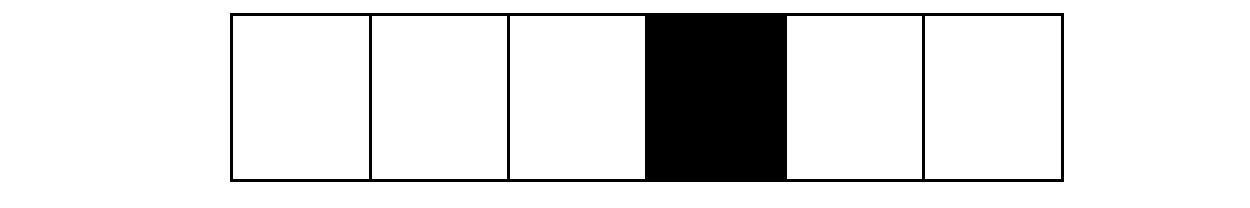
\includegraphics[width=\linewidth]{rkplus_1.png}
  \end{subfigure}
  \begin{subfigure}[t]{.45\linewidth}
    \centering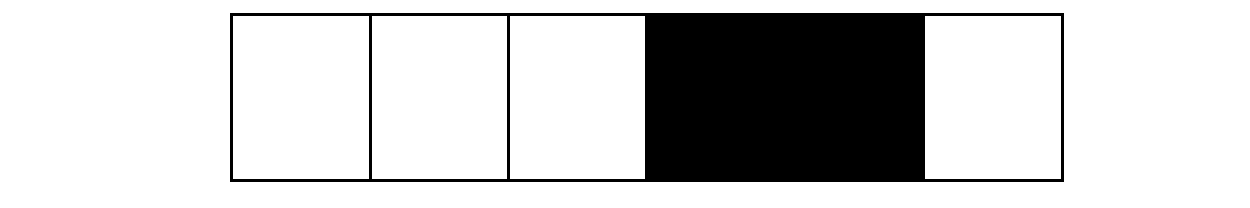
\includegraphics[width=\linewidth]{rkplus_2.png}
  \end{subfigure}
    \begin{subfigure}[t]{.45\linewidth}
    \centering\includegraphics[width=\linewidth]{rkplus_3.png}
  \end{subfigure}
  \begin{subfigure}[t]{.45\linewidth}
    \centering\includegraphics[width=\linewidth]{rkplus_4.png}
  \end{subfigure}
\end{figure}
%\begin{figure}[!htbp]
%\vspace*{-0.25cm}
%\centerline{
%	\subfigure{
%	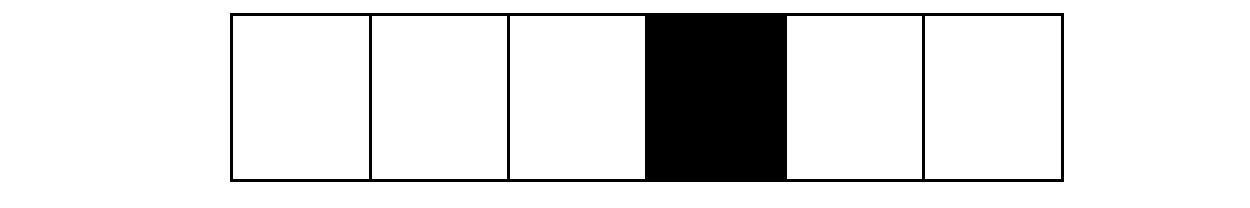
\includegraphics[width=4.0cm]{rkplus_1.png}\hspace*{-0.5cm}}
%		\subfigure{
%	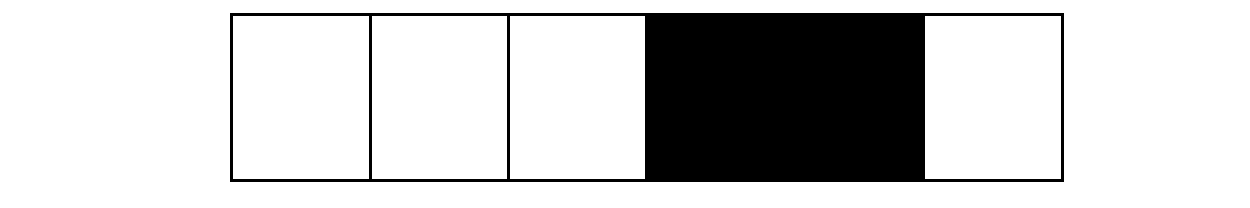
\includegraphics[width=4.0cm]{rkplus_2.png}}
%}
%\centerline{
%	\subfigure{
%	\includegraphics[width=4.0cm]{rkplus_3.png}\hspace*{-0.5cm}}
%		\subfigure{
%	\includegraphics[width=4.0cm]{rkplus_4.png}}
%}
%\end{figure}


%% GENERAL FIGURE
%\begin{figure}
%  \centering
%  \begin{subfigure}[t]{.3\linewidth}
%    \centering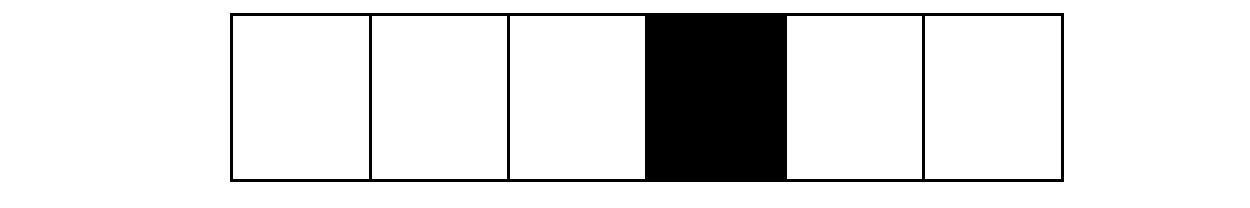
\includegraphics[width=.5\linewidth]{rkplus_1.png}
%    \caption{This is a sub-caption. This is a sub-caption. This is a sub-caption}
%  \end{subfigure}
%  \begin{subfigure}[t]{.3\linewidth}
%    \centering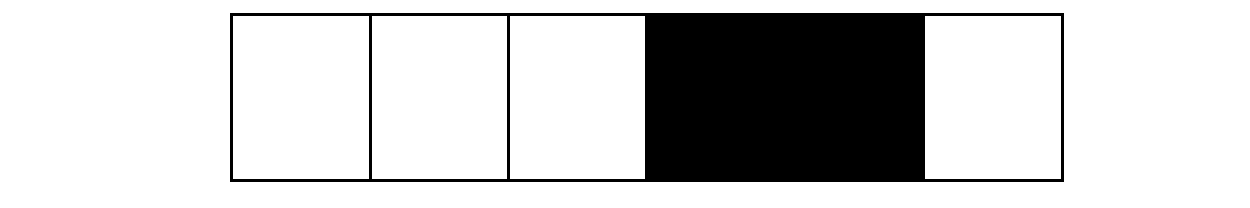
\includegraphics[width=.5\linewidth]{rkplus_2.png}
%    \caption*{This is a sub-caption.}
%  \end{subfigure}
%\end{figure}



\end{frame}




\begin{frame}
\frametitle{Bayesian Update}

\begin{itemize}
	\item Unnormalized Probability:
	\begin{align*}
\tilde P(\mathbf{r}_{k}|z,X_{1:t},Z_{1:t-1})
&=\mathbf{P}_k^-
\bigg[\sum_{i=1}^{k-1}\bigg\{\prod_{j=0}^{i-1}\bar{\mathbf{P}}_j^-\bigg\}p(z|\mathbf{r}_{i+},X_t)\mathbf{P}_k^-\bigg]\nonumber\\
&\qquad + \bigg\{\prod_{j=0}^{k-1}\bar{\mathbf{P}}_j^-\bigg\}p(z|\mathbf{r}_{k+},X_t)\mathbf{P}_k^-
\end{align*}
	\item Normalizer:
	\begin{align*}
\label{eqn:allEta}
\eta
&=
\bigg[\sum_{i=1}^{n_{r}+1}\bigg\{\prod_{j=0}^{i-1}\bar{\mathbf{P}}_j^-\bigg\} p(z|\mathbf{r}_{i+},X_t)\mathbf{P}_k^-\bigg]^{-1}
\end{align*}
	\item Solution: $P(\mathbf{r}_{k}|z,X_{1:t},Z_{1:t-1})=\eta\tilde P(\mathbf{r}_{k}|z,X_{1:t},Z_{1:t-1})$
	\item \emph{Linear Complexity} ($\mathcal{O}(n)$ for \emph{all} $n$ cells in FOV)
\end{itemize}
\end{frame}

\begin{frame}
\frametitle{Complete Update}

\begin{itemize}
	\item 2D and 3D Ray Casting: use geometry to determine which cells a ray intersects and at what depths
	\item Update the grid cells ray-by-ray
\end{itemize}

%% GENERAL FIGURE
\begin{figure}
  \centering
  \begin{subfigure}[t]{.3\linewidth}
    \centering\includegraphics[height=.5\linewidth]{RayCastIllustration.png}
    \caption*{2D Ray Casting}
  \end{subfigure}
  \begin{subfigure}[t]{.3\linewidth}
    \centering\includegraphics[height=.5\linewidth]{test_setup_bottom_left_cropped.jpg}
    \caption*{2D Environment}
  \end{subfigure}
  \begin{subfigure}[t]{.3\linewidth}
    \centering\includegraphics[height=.5\linewidth]{t_end.jpg}
    \caption*{2D Map}
  \end{subfigure}
  \end{figure}
  \begin{figure}
  \centering
%  \vspace*{0.3\linewidth}
  \begin{subfigure}[t]{.3\linewidth}
    \centering\includegraphics[height=.5\linewidth]{experiment_south.jpg}
    \caption*{3D Environment}
  \end{subfigure}
  \hspace*{0.1\linewidth}
  \begin{subfigure}[t]{.3\linewidth}
    \centering\includegraphics[height=.5\linewidth]{experiment_ogm3D_2min47sec.jpg}
    \caption*{3D Map}
  \end{subfigure}
  %
%  \begin{subfigure}[t]{.3\linewidth}
%    \centering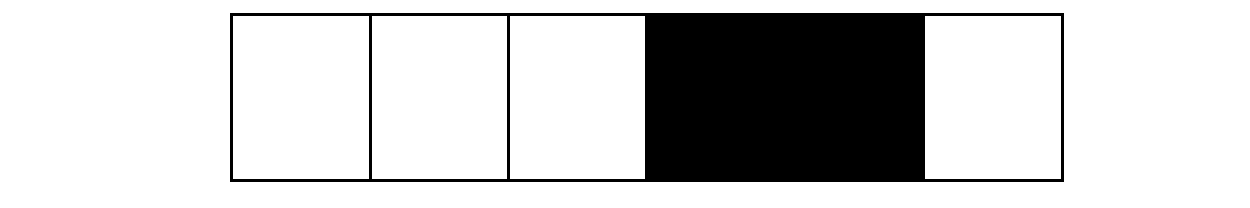
\includegraphics[width=.5\linewidth]{rkplus_2.png}
%    \caption*{This is a sub-caption.}
%  \end{subfigure}
\end{figure}

% RayCastIllustration.png 
% uncomment
%\begin{figure}[!htbp]
%\vspace*{-0.25cm}
%\centerline{
%	\subfigure[Ray Casting]{
%	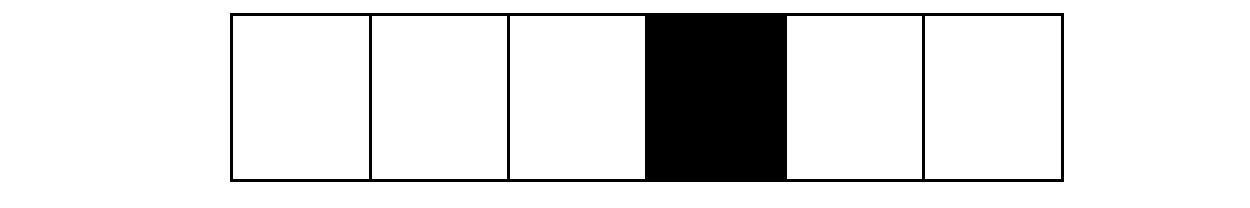
\includegraphics[width=4.0cm]{rkplus_1.png}\hspace*{-0.5cm}}
%		\subfigure{
%	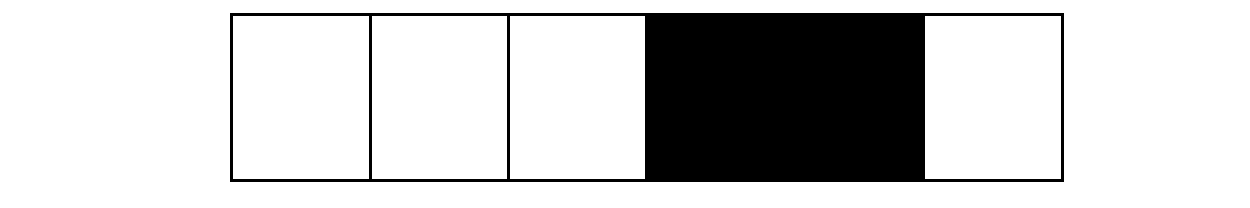
\includegraphics[width=4.0cm]{rkplus_2.png}}
%}
%\end{figure}
\end{frame}

\section*{}
\subsection*{Entropy-Based Exploration}

\begin{frame}
\frametitle{Entropy-Based Exploration}
\begin{itemize}
	\item Existing Approaches
	\vspace*{1cm}
	\item Map Entropy Change
	\vspace*{1cm}
	\item Optimal Pose Selection
	\vspace*{1cm}
	\item Collision-Free Trajectory
\end{itemize}

\end{frame}

\begin{frame}
\frametitle{Existing Exploration Approaches}

\begin{itemize}
	\item Frontier-Based Exploration
	\begin{itemize}
		\item A robot identifies boundaries of free and uncertain cells
		\item The robot moves toward these frontiers, thereby pushing back the boundaries
		\item Heuristic, suboptimal, ad hoc (particularly in 3D)
	\end{itemize}
	\vspace*{0.0cm}\pause
	\item Entropy-Based Approaches
	\begin{itemize}
		\item Probabilities from the occupancy grid map are approximate
		\item Usage of ``hallucination measurements'': assume that $\text{E}[H(P(\mathbf{m}_i|z))]\approx H(P(\mathbf{m}_i|\text{E}[z]))$
	\end{itemize}
	\vspace*{0.0cm}\pause
	\item Proposed Approach
	\begin{itemize}
		\item Use occupancy grid map probabilities
		\item Solve $\text{E}[H(P)]$ and select future poses to maximize map information
		\item Extract important 3D map information into a simplified 2D projected map
	\end{itemize}
\end{itemize}
\end{frame}


\begin{frame}
\frametitle{Expected Information Gain}

\begin{itemize}
	\item Main Idea: determine the benefit of future poses based on how their measurements are expected to improve the map
	\vspace*{0.0cm}\pause
	\item Goal: decrease total map entropy:
	\begin{align*}
		H(P(m))&=\sum_{i=1}^{n_m}H(P(\mathbf{m}_i))
	\end{align*}
	\vspace*{0.0cm}\pause
	\item Measurement Ray Expected Information Gain:
	\begin{align*}
		\text{E}[H(P(m|x_c,z_{c}))]&=\sum_{k=1}^{n_{r}+1}\bigg\{H(P(m|x_c,z_{c,k}))P(z_{c,k}|x_c)\bigg\}
		\\
		P(z_{c,k}|x_c)&=\frac{p(z_{c,k}|x_c)}{\sum_{i=1}^{n_{r}+1}p(z_{c,i}|x_c)}=\frac{\eta_{c,k}^{-1}}{\sum_{i=1}^{n_{r}+1}\eta_{c,i}^{-1}}
		\\
		\mathcal I(x_c,z_{c})&=H(P(m))-\text{E}[H(P(m|x_c,z_{c}))]
	\end{align*}
\end{itemize}

\end{frame}

\begin{frame}
\frametitle{Expected Information Gain Computation}

\begin{itemize}
	\item \emph{Squared Complexity}: $\mathcal O(n_r^2)$ for $n_r$ cells along the ray
	\vspace*{0.0cm}\pause
	\item Two Approaches:
	\begin{itemize}
		\vspace*{0.0cm}\pause
		\item Decrease the cells considered by selecting $n_p$ most probable cells: $\mathcal O(n_r^2)$ reduces to $\mathcal O(n_p^2)$
		\vspace*{0.0cm}\pause
		\item Use 3D cells in a 2D \emph{projection}
\begin{figure}
  \centering
  \begin{subfigure}[t]{.3\linewidth}
    \centering\includegraphics[height=.75\linewidth]{experiment_ogm3D_2min47sec.jpg}
    \caption*{\ \ \ \ \ \ \ \ \ \ \ \ \ \ 3D Map}
  \end{subfigure}
  \hspace*{0.25\linewidth}
  \begin{subfigure}[t]{.3\linewidth}
    \centering\includegraphics[height=.75\linewidth]{experiment_2min47sec.jpg}
    \caption*{2D Projection}
  \end{subfigure}
\end{figure}
	\end{itemize}
\end{itemize}

\end{frame}

\begin{frame}
\frametitle{Map Projection}

\begin{itemize}
	\item Main Idea: choose a cell probability policy incorporating entropy and collision avoidance
		\vspace*{0.0cm}\pause
	\item Consider the 3D cells of $m_C\subset m$ composing the 2D projection:
	\begin{itemize}
		\item If any cell probability $P(\mathbf{m}_i)>P_\text{thresh}$ where $P_\text{init}<P_\text{thresh}<1$, then the projected cell probability is $\text{max}(P(\mathbf{m}_i))$
		\item Otherwise, the projected cell probability is $\text{min}(P(\mathbf{m}_i))$
	\end{itemize}
		\vspace*{0.0cm}\pause
	\item This approach is fairly-conservative for collision avoidance
	\item Relies on the first 3D probabilities that are changed, indicating the true occupancy of the space, even with sparse measurements
	\item Contains information above/below the projected height
	\item Simple and fast: avoids large computations with squared complexities
\end{itemize}

\end{frame}

\begin{frame}
\frametitle{Pose Selection}

\begin{itemize}
	\item Main Idea: select the future pose that maximizes map information gain while accounting for travel distance
	\vspace*{0.0cm}\pause
	\item Attitude Selection: choose the attitude that covers the candidate measurement rays with largest objective function summation
\begin{figure}
\centerline{
	\includegraphics[height=0.35\linewidth]{ExampleOptimalPose.png}
%\begin{picture}(0,0)(0,0)
%\setlength{\unitlength}{0.1\linewidth}\scriptsize
%\put(4.4,2.1){\color{blue}$X_t$}
%\put(5.9,1.9){\color{red}$x_1$}
%\put(2.9,2.0){\color{red}$x_5$}
%\put(4.4,3.6){\color{red}$x_3$}
%\put(4.4,0.6){\color{red}$x_7$}
%\put(5.4,3.0){\color{red}$x_2$}
%\put(3.3,3.1){\color{red}$x_4$}
%\put(3.3,1.0){\color{red}$x_6$}
%\put(5.4,1.0){\color{red}$x_8$}
%\put(6.8,3.1){\color{red}$z_{2,1}$}
%\put(4.5,3.1){\color{red}$z_{2,5}$}
%\put(5.6,4.1){\color{red}$z_{2,3}$}
%\put(5.6,2.2){\color{red}$z_{2,7}$}
%\put(6.5,3.7){\color{red}$z_{2,2}$}
%\put(4.9,3.8){\color{red}$z_{2,4}$}
%\put(5.0,2.5){\color{red}$z_{2,6}$}
%\put(6.5,2.5){\color{red}$z_{2,8}$}
%\put(6.1,2.9){$X_c^*$}
%\end{picture}
}
\vspace*{-0.05\linewidth}
\end{figure}
	\item The attitude $R_c$ is selected for all candidates: the expected information gain becomes $\mathcal I(X_c)$ where $X_c=\braces{x_c,R_c}$
\end{itemize}

\end{frame}





\begin{frame}
\frametitle{Pose Selection}

\begin{itemize}
	\item Travel Distance: generate a cost map from the occupancy grid to obtain distances to each candidate pose $d(x_c)$
	\vspace*{0.0cm}\pause
	\item Bump Function: use a bump function \begin{align*}f(d)=\exp\braces{-\frac{d^2}{2\sigma^2}}+\gamma, \quad \sigma>0, \quad \gamma>0\end{align*} to incentivize the robot to explore more locally until nearby spaces are well-known
	\begin{figure}
	\vspace*{-0.010\linewidth}
\centering
	\includegraphics[width=0.8\linewidth]{GaussianBumpFunFlat.png}
		\vspace*{-0.015\linewidth}
\end{figure}
	% C++: exp(-0.5*distAway*distAway/sigSqrd)+minFunVal GaussianBumpFunFlat.png
	\vspace*{0.0cm}\pause
	\item Select the pose that maximizes the product \begin{align*}X^*=\argmax_{X_c}{\mathcal I(X_c)f(d(x_c))}\end{align*}
\end{itemize}

\end{frame}


\begin{frame}
\frametitle{Collision-Free Path}

\begin{itemize}
	\item Using the cost map from before, \emph{Dijkstra's algorithm} is completed by finding the waypoints from the desired candidate back to the current location
	\vspace*{0.0cm}\pause
	\item These waypoints serve as input to a \emph{constrained polynomial least squares trajectory}
	\begin{itemize}
		\item Each trajectory is solved independently as a function of time, i.e. $x(t)$, $y(t)$
		\item Starting and terminal locations are fixed
		\item Segments patched together have the same position and velocity at the connection
	\end{itemize}
	\vspace*{0.0cm}\pause
	\item A \emph{geometric controller} tracks the trajectory without \emph{singularities} or \emph{ambiguities}
	\vspace*{0.0cm}\pause
	\item The mapping, exploration, and control run in \emph{real-time}
\end{itemize}

\end{frame}

\section*{}
\subsection*{Results}

\begin{frame}
\frametitle{Experimental Setup}
\begin{itemize}
        	\item Hardware
	\begin{itemize}
		\item NVIDIA Jetson Ubuntu computer-on-module
		\item Asus Xtion IR color depth sensor
		\item Hokuyo LIDAR
		\item VectorNav IMU
	\end{itemize}
	\item Software
	\begin{itemize}
		\item Robot Operating System (ROS)
		\item Vicon Tracker (mocap\_vicon)
	\end{itemize}
\end{itemize}
\begin{figure}
  \centering
  \begin{subfigure}[t]{.4\linewidth}
    \centering\includegraphics[height=.5\linewidth]{quad_top.png}
    \caption*{Quadrotor Top}
  \end{subfigure}
  \begin{subfigure}[t]{.4\linewidth}
    \centering\includegraphics[height=.5\linewidth]{quad_bottom.png}
    \caption*{Quadrotor Bottom}
  \end{subfigure}
\end{figure}
\end{frame}

\begin{frame}
\frametitle{Experimental Video}
%\begin{itemize}
%        	\item \href{https://www.youtube.com/watch?v=I_1rXV2XRqk&feature=share}{Video Link}
%\end{itemize}

\begin{figure}[ht]
\includemovie[poster]{0.8\linewidth}{0.45\linewidth}{../../../../Movies/nrl_experiment_narrated.mp4}
\end{figure}



%\only<1->{
%\begin{figure}
%\centering
%\includemovie[poster]{5cm}{6cm}{Farhad_AG.mp4}
%\end{figure}}

%\centering
%\includemedia[
%  width=0.8\linewidth,
%  totalheight=0.45\linewidth,
%  activate=pageopen
%]{\fbox{}}{https://www.youtube.com/watch?v=I_1rXV2XRqk&feature=share}

\end{frame}


\section*{}
\subsection*{Conclusions and Future Work}

\begin{frame}
\frametitle{Conclusions}
\begin{itemize}
        	\item Proposed and tested an occupancy grid mapping technique that uses the \emph{exact probabilistic solution}
	\vspace*{0.0cm}\pause
	\item Computational cost is reduced \emph{substantially} for \emph{real-time implementation} using probabilisitic properties and exploiting mathematical patterns
	\vspace*{0.0cm}\pause
	\item The occupancy grid mapping results are extended to autonomous exploration via expected map entropy changes
	\vspace*{0.0cm}\pause
	\item Dijkstra's search and a constrained polynomial least squares trajectory serves as input for a geometric controller
	\vspace*{0.0cm}\pause
	\item Current and Future Work:
	\begin{itemize}
		\item Multi-vehicle problem: auction-based cooperative approach with receding horizons
		\item Expected entropy of rays through the 3D grid cells
	\end{itemize}
\end{itemize}
\end{frame}






\end{document}

